\def\mytitle{PYTHON PROGRAMMING ON MATRICES}
\def\myauthor{DUDEKULA USENI}
\def\contact{r171099@rguktrkv.ac.in}
\def\mymodule{Future Wireless Communication (FWC)}
\documentclass[10pt, a4paper]{article}
\usepackage[a4paper,outer=1.5cm,inner=1.5cm,top=1.75cm,bottom=1.5cm]{geometry}
\twocolumn
\usepackage{graphicx}
\graphicspath{{./images/}}
\usepackage[colorlinks,linkcolor={black},citecolor={blue!80!black},urlcolor={blue!80!black}]{hyperref}
\usepackage[parfill]{parskip}
\usepackage{lmodern}
\usepackage{tikz}
	\usepackage{physics}
\usepackage{tabularx}
\usepackage{enumitem}
\usetikzlibrary{calc}
\usepackage{amsmath}
\usepackage{amssymb}
\renewcommand*\familydefault{\sfdefault}
\usepackage{watermark}
\usepackage{lipsum}
\usepackage{xcolor}
\usepackage{listings}
\usepackage{float}
\usepackage{titlesec}
\providecommand{\mtx}[1]{\mathbf{#1}}
\titlespacing{\subsection}{1pt}{\parskip}{3pt}
\titlespacing{\subsubsection}{0pt}{\parskip}{-\parskip}
\titlespacing{\paragraph}{0pt}{\parskip}{\parskip}


\newcommand{\myvec}[1]{\ensuremath{\begin{pmatrix}#1\end{pmatrix}}}
\let\vec\mathbf
\lstset{
frame=single, 
breaklines=true,
columns=fullflexible
}
\thiswatermark{\centering \put(0,-110.0){
\includegraphics[scale=0.3]{logo.png}} }
\title{\mytitle}
\author{\myauthor\hspace{1em}\\\contact\\FWC220\hspace{6.5em}IITH\hspace{0.5em}\mymodule\hspace{6em}Matrix:Circle}
\date{}
\begin{document}
	\maketitle
	\tableofcontents
   \section{Problem}
  From the origin, chords are drawn to the circle 
$(x-1)^2 + y^2=1$., find the equation of the locus of the mid-points of these chords
\section{Construction}
 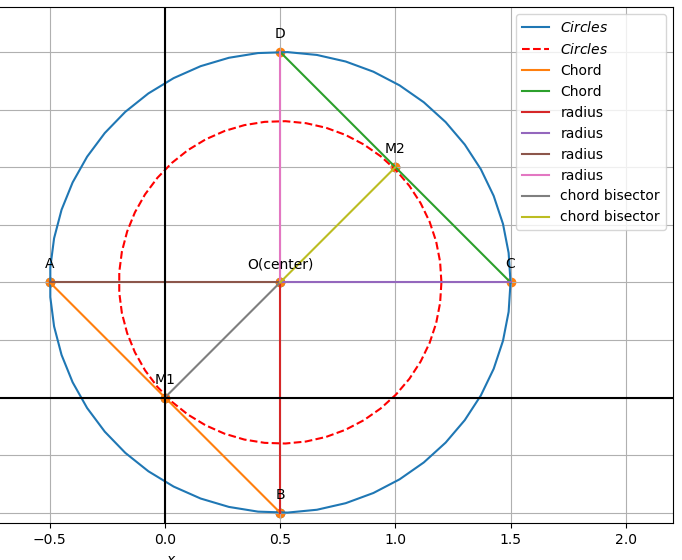
\includegraphics[scale=0.3]{cic1.png}
  	\begin{center}
  Figure of construction
  	\end{center}
  \section{Solution}

Circle equation : $(x-1)^2+y^2=1$\\
The standard equation of the conics is given as :
\begin{align}
\vec{x}^{\top}\vec{V}\vec{x}+2\vec{u}^{\top}\vec{x}+f=0
\end{align}
The given circle  can be expressed as conics with \\parameters
\begin{align}
	\vec{V} &= \vec{I}, \vec{u} = -\myvec{-1 \\0}, f = 0
	\end{align}

	Radius and Centre are
	\begin{align}
	r &=\sqrt{{\vec{u}^{\top}\vec{u}}-f },\vec{C}=-u
    \end{align}
\begin{equation}
  r=1 
\end{equation}
From the figure
\begin{align}
    \vec{A}^{\top}\vec{B}=0
\end{align}
Let $\vec{R}$ is the rotation matrix of given circle  \\\vspace{1mm}
\begin{align}
 \vec{R} = \myvec{0 & -1 \\1 & 0}
\end{align}

Let $\vec{B}$ be the another end point of chord \\\vspace{1mm}
\begin{align}
    \vec{B} = \vec{RA}
\end{align}
Let $\vec{P}$ be th mid point of chord of the circle
\begin{align}
    \vec{P} = \frac{\vec{A+B}}{2}
\end{align}
\begin{align}
     \vec{P} = \frac{\vec{A+RA}}{2}
\end{align}
\begin{align}
     \vec{P} = \frac{\vec{A(I+R)}}{2}
\end{align}
\begin{align}
     \vec{A} =\vec{\vec{2P[I+R]}}^{-1}
\end{align}

STEPS TO FIND THE LOCUS OF THE MIDPOINT OF CHORD OF THE CIRCLE:\\
By substituting $\vec{A}$ value in quadratic form of the circle we get
\begin{align}
\vec{[2P(I+R)}^{-1}]^{\top}[\vec{2P(I+R)}^{-1}]+2[\vec{2P(I+R)}^{-1}]\myvec{\vec{u}}^{\top}+0=0
\end{align}
$$\vec{P}^{\top}\vec{[2(I+R)}^{-1}]^{\top}\vec{P}\vec{[2(I+R)}^{-1}]+4\vec{P}[\vec{(I+R)}^{-1}]\myvec{\vec{u}}^{\top}+0=0$$
\begin{align}
\vec{P}^{\top}\vec{V}\vec{P}+2\vec{u}^{\top}\vec{P}+0=0\\
 \vec{V}=\vec{I} ,\vec{u}^{\top}=(-0.5 -0.5)
\end{align}
Finally  Equation of the locus of the midpoint  of  chord of the given circle:
\begin{align}
\vec{P}^{\top}\vec{V}\vec{P}+2\vec{u}^{\top}\vec{P}=0
\end{align}
\begin{align}
\vec{X}^{\top}\vec{V}\vec{X}+2\vec{u}^{\top}\vec{X}=0
\end{align}

\section{Software}
\begin{center}
 \begin{lstlisting}
Below python code realizes the above construction :
https://github.com/dudekulauseni123/FWC0982022
 \end{lstlisting}
\end{center}
\end{document}
